\subsection{Airfoil Analysis}
The desired cruise conditions of Mach $= 0.9$ for the aircraft fall within the transonic speed regime.  This provides favorable conditions for the sizing analysis but increases the effects of wave drag.

\begin{wrapfigure}{r}{0.5\textwidth}
    \vspace{-0.25in}
    \centering
    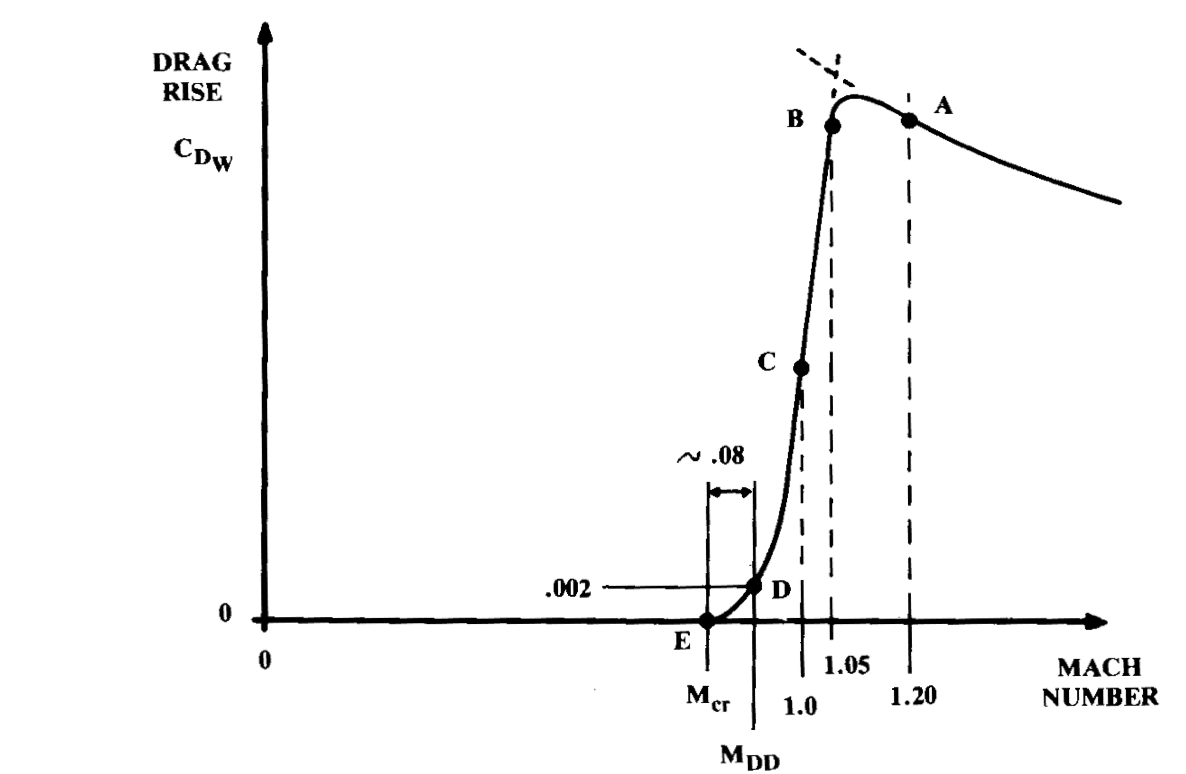
\includegraphics[width=0.5\textwidth]{Photos/wavedragduetotransonic.png}
    \caption{Wave Drag due to Transonic Airspeed\\{\small From Raymer Fig. 12.29\cite{raymer}}}
    \label{fig:transonic}
    \vspace{-0.5in}
\end{wrapfigure}

As shown above in Figure \ref{fig:transonic}, there is an increase in wave drag as Raymer's example aircraft passes into the transonic regime.  Therefore, a selection of supercritical airfoils and wing sweep of no less than $32\degree$ is proposed in mitigation of the above trend.  To properly predict and quantify the wave drag for aerodynamic analysis on the airfoil and wing design, \textit{Method B} from Vargas\cite{vargas} shall be included in the part-by-part drag buildup.  The supercritical airfoils tested for analysis include the following from Selig's Airfoil Database:

\begin{table}[!h]
    \centering
    \caption{Airfoil Options}
    \begin{tabular}{|c|c|} \toprule
        \textbf{Airfoil Type} & \textbf{Priority} \\ \hline \hline
        SC(2)-0412 & 1 \\ \hline
        SC(2)-0714 & 2 \\ \hline
        SC(2)-0612 & 3 \\ \hline
    \end{tabular}
    \label{tab:my_label}
\end{table}

Several SC(2)-series airfoils are compared using incompressible methods on XFLR5.  These methods do not offer accurate analysis of the fluid behavior at transonic cruise conditions but provides initial guidance as to selecting an airfoil.
% \clearpage %-- this gets Perf to be almost perfectly on the top of a page.  Please advise. 

\subsection{Wing Design}
Initial assumptions were made for the aspect ratio of the wing design based on comparable aircraft such as the Boeing 777-200 and Boeing 787.  Consequently, a range of $\AR \in [8,12]$ was initially set.  A wing area of $5,000 \text{ ft}^2$ was recommended from the performance analysis.  Later analysis proved better range performance with a wing reference area of $4,000 \text{ ft}^2$. The modified wing dimensions are shown to the below in Table \ref{tab:wingsizing}.

\begin{table}[!h]
    \centering
    \caption{Wing Dimensions}
    \begin{tabular}{|c|c|c|} \toprule
        \multicolumn{3}{c}{\textbf{\textcolor{cobalt}{Main Wing}}} \\ \midrule
        \textbf{Description} & \textbf{\#} & \textbf{Units} \\ \hline \hline
        \AR & 8.5 & $\sim$ \\ \hline
        b (\textit{span}) & 184 & ft \\ \hline 
        $S_{\text{wing}}$ (\textit{area}) & 4,000 & ft$^2$ \\ \hline
        c/4 Sweep & $32$ & degree \\ \hline
        $\lambda$ & 0.15 & $\sim$ \\ \hline
        Chord Root & 452.72 & in \\ \hline
        Chord Tip & 67.91 & in \\ \hline   
        Mean Aerodynamic Chord & 307.72 & in \\ \bottomrule
    \end{tabular}
    \label{tab:wingsizing}
\end{table}

\subsection{Drag Buildup}
The Drag for Sam Mark I. is built up part-by-part by separating the fuselage, wings, empennage, and other protuberances and calculating the following seven key forms of drag, shown in Equation \ref{eqn:drag_general}:
\begin{equation}\label{eqn:drag_general}
    C_D = C_{D,0} + C_{D,i} + C_{D,W_{NL}} + C_{D,W_{L}} + C_{D_{EXCR}} + \Delta C_{D_{Re}} + C_{D,trim}
\end{equation}

The increased effects of wave drag experienced during transonic flight are calculated by using the proposed Method B from Vargas.  This method accounts for the use of supercritical airfoils by offsetting the McDevitt method by adding the Torenbeek method.


\subsection{High-Lift Systems}
High-lift devices are implemented on Sam Mark I to improve aircraft stability during take-off and landing segments of the mission profile.  Leading edge slats and trailing edge Fowler flaps are included on the wing.  The dimensions, mechanisms, aerodynamic characteristics, and stability will be part of a future analysis.

\subsection{Future Progress}
Several key topics are under active investigation to improve the aircraft performance. The following will be further investigated for the Preliminary Design Report:
\begin{itemize}
    \item Complete Drag Buildup (Major focus on Wave drag prediction)
    \item High lift devices during Take-off/Landing, Lift-Drag Polar, and impact of flaps and slats on aircraft stability
    \item XFLR5 Analysis of Supercritical Airfoils to determine desired airfoil
    \item Wing geometry with airfoil design
    \item CFD analysis of complete wing and body system
\end{itemize}


% \textcolor{red}{
% \begin{itemize}
%     \item Discuss wing design, including reasoning. \checkmark JJ
%     \item Discuss high-lift system, including reasoning. \checkmark JJ
%     \item Discuss drag buildup (tabulated) used to support sizing analysis. \checkmark JJ
%     \item Discuss future work. X
%     \item AIAA: Important aerodynamic characteristics and aerodynamic performance for key mission
%     segments and requirements (shared w/ aero) N/A for now \checkmark
% \end{itemize}}